\scanpage{50}%
\mspage{\handwritten{18}}%
rien, il s'ensuit que l'un des $K_i$ est déjà réduit au groupe unité, donc que $G\handwritten{\to}\underline{\operatorname{Aut}}_{\inserted{\handwritten{V_i}}}\deleted{\unsure{(V_i)}}$ est un monomorphisme. C'est donc une immersion fermée en vertu de (1.4.2), ce qui prouve que (iv)$\handwritten{\Rightarrow}$(v). Comme (\deleted{\unsure{g}}v)$\handwritten{\Rightarrow}$(i) trivialement, cela prouve 11.11\deleted{\unsure{.}} pour $G$ de type fini.

\deleted{Prenons maintenant le cas général, où il reste à prouver que (iv)$\handwritten{\Rightarrow}$(i). Avec les notations de la démonstration précédente, soit $G_i$ le\inserted{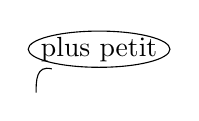
\begin{tikzpicture}[x=1cm,y=1cm,baseline=(n.base)]\node (n) at (0,0) {plus petit};\draw (0,0) ellipse (.9 and .23);\draw (-.6,-.25) .. controls (-.8,-.2) and (-.8,-.4) .. (-.8,-.55);\end{tikzpicture}} sous-groupe fermé de $\operatorname{Aut}(V_i)$ par lequel\inserted{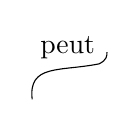
\begin{tikzpicture}[x=1cm,y=1cm,baseline=(n.base)]\node (n) at (0,0) {peut};\draw (-.45,-.65) .. controls (-.5,-.2) and (-.1,-.3) .. (.4,-.2) .. controls (.5,-.15) and (.5,-.1) .. (.5,-.05);\end{tikzpicture}} se factoriser $G\handwritten{\to}\underline{\operatorname{Aut}}_{\inserted{\handwritten{V_i}}}\deleted{(V_i)}$ \deleted{(existe} (un tel groupe existe, \deleted{puisque} comme intersection de tous ceux par lesquels se factorise $G\handwritten{\to}\deleted{\unsure{\operatorname{Aut}(V_i)}}\inserted{\underline{\operatorname{Aut}}_{V_i}}$). Si $V_j\handwritten{\supset}V_i$, on voit alors tout de suite que $G_j$ invarie $V_i$ , et que le morphisme correspondant $G_j\handwritten{\to}\underline{\operatorname{Aut}}_{V_i}$ se factorise par $G_i$ . De cette façon, les $G_i$ forment un système projectif de groupes affines sur $k$, et on a un morphisme naturel $G\handwritten{\longrightarrow}G'=\underset{\handwritten{\longleftarrow}}{\lim}G_i$ , où $G'$ est lui-même un groupe affine (EGA IV 8.2.3). L'hypothèse que $G$ opère \uline{fidèlement} sur $V$ s'exprime alors par\deleted{\unsure{r}} le fait que $G\handwritten{\to}G'$ est un monomorphisme. On a donc trouvé\handwritten{\makebox[0pt][l]{\raisebox{-.5ex}{\begin{tikzpicture}[x=.25cm,y=.25cm]\draw (0,-.5)--(.55,1);\end{tikzpicture}}}}un monomorphisme de $G$ dans un schéma affine, ce qui implique que le schéma quasi-compact\inserted{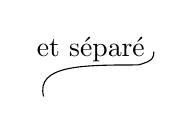
\begin{tikzpicture}[x=1cm,y=1cm,baseline=(n.base)]\node (n) at (0,0) {et séparé};\draw (-.6,-.6) .. controls (-.7,-.2) and (-.1,-.2) .. (.6,-.2) .. controls (.8,-.15) and (.8,-.1) .. (.8,-.03);\end{tikzpicture}} $G$ est quasi-affine, i.e. que son faisceau structural est ample, en vertu de EGA IV 18.12.17 . En \handwritten{d}'autres termes, posant $H=\operatorname{Spec}\handwritten{\Gamma}(G,\underline{O}_G)$ , le morphisme canonique $G\handwritten{\to}H$ est une immersion ouverte. Notons maintenant que $H$ est de façon naturelle un schéma en groupes, et $G\handwritten{\to}H$ un homomorphisme de groupes, grâce à 11.2 . Cet homomorphisme est évidemment dominant, il reste à prouver que c'est un isomorphisme, ce qui résulte\deleted{ra de} du lemme suivant:}
\margin{\handwritten{\figure{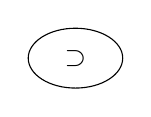
\begin{tikzpicture}
\draw (0,0) ellipse (.6 and .38);\node at (0,0) {$\supset$};
\end{tikzpicture}}}}

\deleted{\uline{Lemme} 11.11.1.\handwritten{\unsure{,}} Soient $\deleted{\unsure{G}}\handwritten{H}$ un schéma en groupes sur un corps\inserted{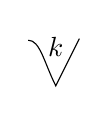
\begin{tikzpicture}[x=1cm,y=1cm,baseline=(n.base)]\node (n) at (0,0) {$k$};\draw (-.35,.08) .. controls (-.2,.08) and (-.15,-.2) .. (0,-.5)--(.3,.1);\end{tikzpicture}}\handwritten{.} \deleted{$G$ un sous-} Alors tout sous-schéma en groupes ouvert\inserted{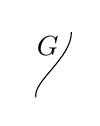
\begin{tikzpicture}[x=1cm,y=1cm,baseline=(n.base)]\node (n) at (0,0) {$G$};\draw (.3,.18) .. controls (.3,-.15) and (-.2,-.45) .. (-.15,-.65);\end{tikzpicture}} de $H$ est aussi fermé.}
\margin{\handwritten{\figure{\begin{tikzpicture}\draw (0,0)--(.03,-.8);\end{tikzpicture}}}}

\deleted{Il revient au même de dire que l'ensemble $H-G$ est ouvert, i.e. est un voisinage de chacun de ses points\deleted{,} $x$ . Or , toute extension de corps $k'/k$ définissant un morphisme $\operatorname{Spec}k'\handwritten{\to}\operatorname{Spec}k$ qui est universellement}
% archive sheet number: 49
